\documentclass{article}
\usepackage{amsmath}
\usepackage{siunitx}
\usepackage{graphicx}
\usepackage{booktabs}
\usepackage{wrapfig}
\usepackage[italian]{babel}
\usepackage[tmargin=2cm,rmargin=1.5in,lmargin=1.5in,margin=0.85in,bmargin=2cm,footskip=.2in]{geometry}
\usepackage{siunitx}
\sisetup{separate-uncertainty=true, per-mode=fraction, parse-numbers=true}
\usepackage{caption}
\usepackage[T1]{fontenc}
\usepackage{bookmark}
\usepackage{mathcomp}
\usepackage{graphicx}
\usepackage{multicol}
\usepackage{booktabs}
\usepackage{amsmath,amsfonts,amsthm,amssymb,mathtools}
\hypersetup{
	pdftitle={Relazione pendolo fisico},
	colorlinks=true, linkcolor=doc!90,
	bookmarksnumbered=true,
	bookmarksopen=true
}
\usepackage{blindtext}
\usepackage{wrapfig}
\usepackage{listings}
\usepackage{xcolor}
\usepackage{float}
\usepackage{tikz}
\usepackage{multirow}
\usepackage{biblatex}
\definecolor{codegreen}{rgb}{0,0.6,0}
\definecolor{codegray}{rgb}{0.5,0.5,0.5}
\definecolor{codepurple}{rgb}{0.58,0,0.82}
\definecolor{backcolour}{rgb}{0.95,0.95,0.92}
\definecolor{doc}{rgb}{0,0,0}
\lstdefinestyle{code}{
    backgroundcolor=\color{backcolour},   
    commentstyle=\color{codegreen},
    keywordstyle=\color{magenta},
    numberstyle=\tiny\color{codegray},
    stringstyle=\color{codepurple},
    basicstyle=\ttfamily\footnotesize,
    breakatwhitespace=false,         
    breaklines=true,                 
    captionpos=b,                    
    keepspaces=true,                                     
    showspaces=false,                
    showstringspaces=false,
    showtabs=false,                  
    tabsize=2,
    inputencoding=ansinew,
    extendedchars=true,
    numbers=left,                    
    numbersep=5pt
}

\lstset{style=code}
\usepackage[varbb]{newpxmath}
\usepackage{circuitikz}
\captionsetup{labelfont={bf, sc}}
% Prima cosa che mi ha puntualizzato Baldini è il fatto che noi qua misuriamo g non lo calcoliamo: io avevo scritto "Relazione calcolo di $g$" ma qua lo stiamo misurando alla fine, non calcolando da una serie di principi primi
\title{Relazione misura di $g$}
\author{Francesco Sermi}
\date{\today}

\begin{document}
\maketitle

\section{Scopo dell'esperienza}
Misura dell'accelerazione di gravità $g$ tramite una molla.

\section{Premesse teoriche}
Una molla è un corpo in grado di allungarsi e accorciarsi se gli viene applicata una forza e in seguito di ritornare alla propria forma naturale. Tramite la legge di Hooke sappiamo che essa reagisce esercitando una forza che reagisce alle sollecitazioni subita longitudinalmente, in trazione o in compressione, lungo un asse $\hat{x}$
\begin{equation}
\vec{F_e} = - k \Delta l \hat{x}
\end{equation}
quindi si osserva che essa è direttamente proporzionale all'allungamento o alla compressione $\Delta l$ (che dimensionalmente ha come unità di misura quella di una lunghezza $[L]$) della molla dovuto alla sollecitazione e la costante di questa proporzionalità $k$ si chiama \emph{costante elastica della molla} (che invece dimensionalmente ha l'unità di misura di una forza diviso una lunghezza, dunque $\frac{[L][T]^{-2}[M]}{[L]} = [M][T]^{-2}$). \\
La forza di gravità esercitata dalla Terra su un corpo che si trova sulla sua superficie è pari a
$\vec{F} = m\vec{g}$
dove $\vec{g}$ è l'accelerazione di gravità sulla superficie terrestre. È possibile stimare il valore di $g=|\vec{g}|$ misurando l'allungamento della molla dovuto all'azione di una massa appesa ad una estremità della molla, pertanto:
\begin{equation}
	m_i|\vec{g}| = k \Delta l \implies |\vec{g}| = \frac{k}{m_i} \Delta l = \frac{k}{m_i} (l_f - l_0)
	\label{secondo_modello}
\end{equation}
Non deve sorprendere il fatto che in questa formula non compaia la massa della molla siccome è tenuta di conto dentro $l_0$ siccome ho misurato la lunghezza a riposo della molla quando essa era già sospesa al supporto, quindi si tiene già di conto della sua massa.
Tramite una stima della lunghezze $\Delta l$, $k$ e conoscendo la massa $m_i$ appesa possiamo stimare $g$. Per fare ciò, ci avvarremo della formula del periodo $T$ delle oscillazioni compiute dalla molla con la massa appesa
\begin{equation}
	T = 2 \pi \sqrt{\frac{m_i+\frac{m_m}{3}}{k}}
	\label{primo_modello}
\end{equation}
dove è interessante notare il fatto che compare il termine $\frac{m_m}{3}$ che tiene di conto della massa della molla, che non è trascurabile.

\section{Apparato sperimentale}
Non ho ancora capito quando è sensibilità e quando risoluzione
\textbf{Strumenti}:
\begin{itemize}
	\item metro a nastro con sensibilità pari a $0.1 \si{\centi\meter}$
	\item cronometro con risoluzione pari a $0.001 \si{\second}$
	\item bilancia di precisione con sensibilità pari a $0.001 \si{\gram}$
\end{itemize}		
\textbf{Materiali}:
\begin{itemize}
	\item supporto per la sospensione della molla
	\item pesini di metallo di masse differenti
	\item piattino di metallo
	\item molla
\end{itemize}

\section{Descrizione delle misure}
Prima di procedere abbiamo misurato la massa del piattino, che risultava essere pari a $m_p = (7.874 \pm 0.001) \si{\gram}$ e la massa della molla, pari a $m_m = (8.093 \pm 0.001) \si{\gram}$. \\
Successivamente abbiamo effettuato le misure necessarie per stimare la costante elastica della molla $k$, misurando le oscillazioni della molla soggetta alla forza peso esercitata dalla massa del piattino e di un pesino posto sopra utilizzando varie masse, che riportiamo in una tabella qua accanto. \\

\begin{wraptable}{r}{0.4\textwidth}
	\centering
	\begin{tabular}{c c}
	\toprule
	$m_i \, [\si{\gram}]$ & $T_i \, [\si{\second}]$ \\
	$\pm 0.001$ &  \\
	\midrule
	$10.652$ & $0.575 \pm 0.009$ \\
	$28.945$ & $0.751 \pm 0.005$ \\
	$16.541$ & $0.625 \pm 0.003$ \\
	$4.694$ & $0.52 \pm 0.01$ \\
	$34.956$ & $0.961 \pm 0.009$ \\
	\bottomrule		
	\end{tabular}
	\caption{Tabella con le misure del periodo di oscillazione per ogni pesino di massa $m_i$ attaccato alla molla}
\end{wraptable}

\noindent Siccome la misura di ogni oscillazione è soggetta ad errori accidentali dovuti al mio tempo di reazione nel fermare il cronometro, per ogni massa ho misurato $10$ volte il periodo di oscillazione e, successivamente, come risultato della nostra misura abbiamo preso per il pesino $i$-esimo:
$$
\hat{T_i} = T_{m_i} \pm \sqrt{\frac{1}{10 \cdot 9} \sum_{j=1}^{10} (T_j - T_{m_i})^2}
$$
dove $T_{m_i}$ rappresenta la media aritmetica di tutti i periodi di oscillazione che abbiamo misurato per l'$i$-esimo pesino e $T_j$ rappresenta invece il $j$-esimo valore misurato per l'$i$-esimo pesino. \\
Successivamente, ho misurato gli allungamenti $\Delta_l$ della molla con pesini di masse diverse: inizialmente ho misurato $l_0 = (11.3 \pm 0.1) \si{\centi\meter}$ e, siccome $\Delta l_i = l_f - l_0$, come errore sugli allungamenti ho sommato in quadratura gli errori su $l_f$ e $l_0$:
$$
\sigma_{\Delta_l} = \sqrt{\sigma_{l_f}^2 + \sigma_{l_0}^2}
$$
Riportiamo nella tabella qua sotto le misure:
\begin{table}[H]
	\centering
	\begin{tabular}{c c}
	\toprule
	$m_i \, [\si{\gram}]$ & $\Delta l \, [\si{\meter}]$ \\
	$\pm 0.001$ & \\
	\toprule
	$10.652$ & $0.08 \pm 0.01$ \\
	$28.945$ & $0.16 \pm 0.01$ \\
	$16.541$ & $0.102 \pm 0.01$ \\
	$4.694$ & $0.05 \pm 0.01$ \\
	$34.956$ & $0.18 \pm 0.01$ \\
	\bottomrule
	\end{tabular}
	\caption{Tabella con gli allungamenti $\Delta l_i$ della molla per ogni pesino di massa $m_i$}
\end{table}
\section{Analisi delle misure}
Per effettuare la stima della costante elastica $k$ della molla ho deciso di farmelo stimare tramite la procedura del fit dei minimi quadrati tenendo $k$ come parametro libero e utilizzando come modello la (\ref{primo_modello}). Si riporta il grafico di best-fit qua sotto:

\begin{figure}[H]
	\centering
	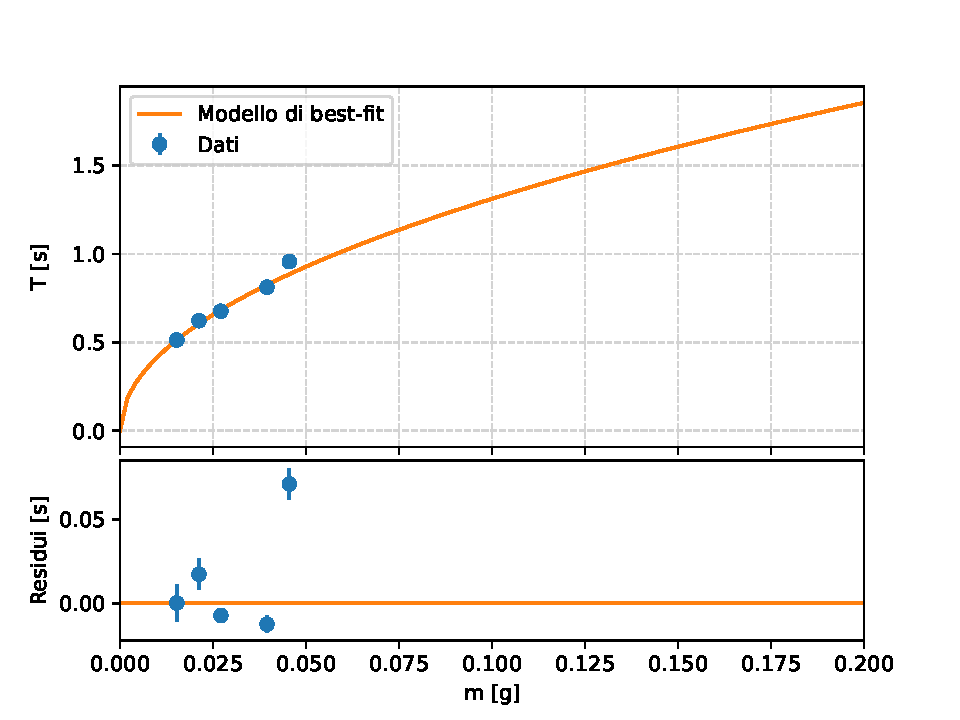
\includegraphics[scale=0.50]{Modello_best_fit_k_residui.pdf}
	\caption{Grafico di best-fit del modello \ref{secondo_modello}}
\end{figure}


\noindent La funzione \texttt{curve\_fit} di \texttt{scipy} restituisce che la costante elastica della molla ha il seguente valore $\hat{k} = (2.27 \pm 0.07) \si{\newton\per\meter}$. 
Effettuando il test del $\chi^2$, si osserva che il $\chi^2$ restituito dal fit è $\chi^2 \approx 76$, un valore che si trova ben oltre una deviazione standard del $\chi^2$ atteso con il mio numero di gradi di libertà. \\
LEGGERE COMMENTI IN CODICE \LaTeX
%
% COMMENTO: Qua sotto avevo deciso di calcolarmi $g$ per ogni massettina, il problema è che, utilizzando k stimato dal fit, si fa in modo che i valori diventino in qualche modo dipendenti siccome hanno una componente di errore che è la stessa diciamo, quindi 
%è proprio sbagliata l'idea di fit fatta in questa maniera siccome si richiede che le misure siano indipendenti
%
% VECCHIA RELAZIONE:
%\noindent Come errore sui vari $g_i$ ho propagato gli errori delle grandezze coinvolte nella (\ref{secondo_modello}), osservando che
%$$
%\frac{\sigma_{g_i}}{g_i} = \sqrt{\left( \frac{\sigma_k}{k} \right)^2 + \left(\frac{\sigma_m}{m} \right)^2 + \left(\frac{\sigma_{\Delta l}}{\Delta l} \right)^2 } \implies \sigma_{g_i} = g_i \sqrt{\left( \frac{\sigma_k}{k} \right)^2 + \left(\frac{\sigma_m}{m} \right)^2 + \left(\frac{\sigma_{\Delta l}}{\Delta l} \right)^2 }
%
%\noindent Per determinare $g$ abbiamo invece deciso di effettuare sempre un'analisi tramite fit dei minimi quadratici tenendo $g$ come parametro libero, riportando i valori $g_i$ calcolati con la (\ref{secondo_modello}) in un grafico $g_i - m_i$ e fittando con una retta del tipo $y=c$, che riportiamo qua sotto:

%\begin{figure}[h]
%	\centering
%	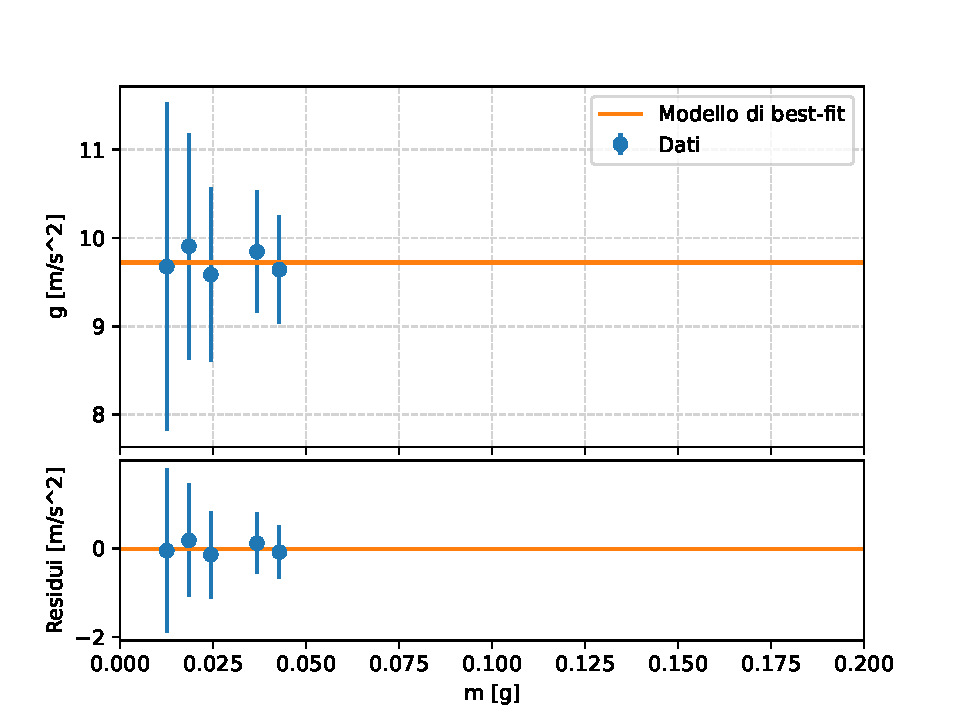
\includegraphics[scale=0.60]{Modello_best_fit_residui_g.pdf}
%\end{figure}

%A questo punto si procede andando a stimare dal fit il parametro $\frac{g}{k}$ utilizzando le posizioni di equilibrio e subito dopo, moltiplichiamo per il $k$ stimato dal precedente fit per ricavare $g$ (LEGGERE COMMENTI NEL CODICE \LaTeX).

\section{Conclusioni}
% VECCHIA RELAZIONE:
%
%Il parametro $g$ stimato dalla funzione \texttt{curve\_fit} risulta essere pari a $\hat{g} = (9.72 \pm 0.06) \si{\meter\per\second^2}$ che non è compatibile entro le barre di errore con il valore atteso, siccome, in corrispondenza della superficie terrestre, questo risulta essere pari a $g=9.81 \si{\meter\per\second^2}$. Il motivo di tale discrepanza, dato il $\chi^2$ elevato potrebbe essere dovuto al fatto che nell'esperienza hanno influito delle fonti di errori sistematici che non sono stato in grado di rilevare oppure ho sottostimato gli errori sulle oscillazioni della molla (in particolar modo nei pesini con una massa molto piccola dove la frequenza di oscillazione era elevata e potrei aver tenuto di conto di una oscillazione in più).
\end{document}
